\chapter{Classification of Cellular Automata based on Hamming distance}
\label{chap:HammingECA}

\renewcommand\labelenumi{(\roman{enumi})}
\renewcommand\theenumi\labelenumi


\begin{quotation}
	\vspace{-3cm}
    \begin{flushright}
    \begin{minipage}[t][5cm][b]{0.5\textwidth}
    {\letquote ``Automation is good, so long as you know exactly where to put the machine."}
    
    \bigskip
    
    -{\small  Eliyahu Goldratt}
    \end{minipage}
    \end{flushright}
    
    \vspace{0.5cm}
\end{quotation}

\vspace{0.5cm}

\let\thefootnote\relax\footnotetext{
%\bibitem{Alfaro2024}
G. Alfaro and M. A. F. Sanjuán,
Classification of cellular automata based on the Hamming
distance,
Chaos \textbf{34}, 083129 (2024)\\
\url{https://doi.org/10.1063/5.0227349}
}

\vspace{1cm}


In the previous chapter we reviewed evolutionary social games and configured them for agents to play in a square lattice with their neighbors. We calculated the payoff of each individual according to some rules and then they adopted the strategy of one of its neighbors depending on the payoff. Since the payoff of the agents depends only on the state of their neighbors, if we do not allow error of decision (i.e. with the decision-making Rule-$K \to 0$), then each combination of neighboring agents will produce unambiguously the updated state of the central agent at the next iteration. Therefore, if we have the prisoner's dilemma with Moore neighborhood as in last chapter, the state of an agent depends only on the state of all its $24$ neighbors and its own. 

One could obtain all of the possible results of the game with the different combinations of these $25$ agents. Given that each agent can only be either a cooperator or a defector, we get $2^{25}$ different situations that completely define the system. If now we would get the state of the current cell at the next iteration for each of these situations, then we would have formalized the game as a cellular automaton. The rules of this automaton would be each of the combinations of the neighborhood cells states. That would be $2^{25}$ rules to follow, which would make a very complicated cellular automaton, although one could get the same behavior with a lower number of rules by intelligently making more complicated rules. 

For this study we use the algorithm developed in the investigation of the previous chapter, but this time with implement it on elementary cellular automata, the most simple cellular automata.

But, what exactly is a cellular automaton?

\section{Introduction}


A cellular automaton, or CA, is a collection of rules that determine the dependence of cells' states to the state of neighboring cells.
Usually, CA do not have a rule for every combination of states of cells, but have a few rules that univocally tells each cell how to update. Take for example Conway's Game of Life. With only four rules that check weather a certain number of neighboring cells are alive or dead, (1 or 0), the state of each cell is determined. With only these four rules the system presents a broad complexity, with complex patterns arising from simple initial configurations. 


There are different methods to increase the complexity of cellular automata. One could let the cells have more than two states, like the first ever studied cellular automata, which was developed in the late 1950s by John von Neumann~\cite{VonNeummanCA} and had 29 states per cell. It was developed as a model for discrete liquid motion, but he was also interested in the idea of self-replication and how machines could replicate themselves. With this automata he made a universal constructor. Additionally increasing the spatial dimensions of the system would complicate the dynamics. One could also let the automata have memory by allowing the rules to depend on the state of cells at previous iterations.

This complexity arising from simple rules has given rise to the thorough research of CA in many ambits of science. For example, in physics they have been used to model the circulation of vehicles,~\cite{PhysicsCA1}, and pedestrians~\cite{PhysicsCA2}. In~\cite{PhysicsCA3} a model for discrete lattice gases are cellular automata. The authors of~\cite{PhysicsCA4} use a set of cellular automata to simulate avalanches in sand piles. Cellular automata has also been used in quantum mechanics,~\cite{PhysicsCA5}. They have also been studied in engineering to implement logical devices as in~\cite{EngineeringCA1}. In cryptography they are widely used as in~\cite{CryptographyCA1, CryptographyCA2Lya}. Multiple applications have also been found in biology,~\cite{BiologyCA1, BiologyCA2, BiologyCA3}


To measure this complexity we will use, again, the Hamming distance, but in order of understanding better the limitations of this distance for measuring complexity, here we study the simpler case of CA, the Elementary Cellular Automata, or ECA. 







\begin{table}
\centering
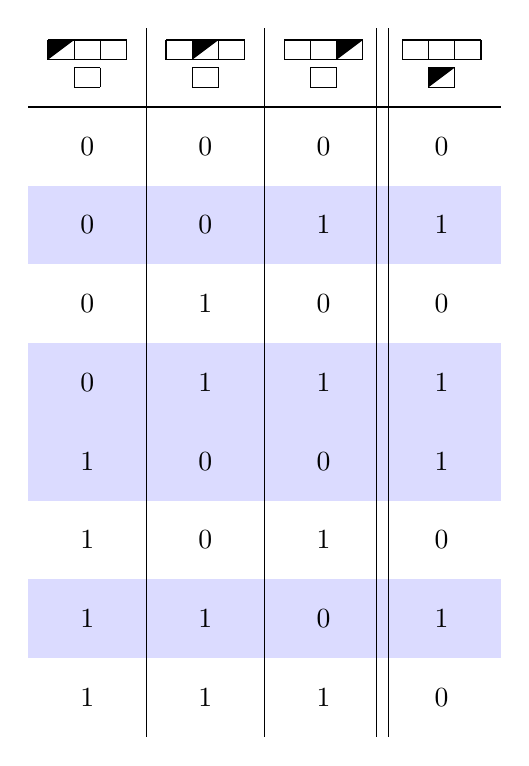
\begin{tikzpicture}

%color

\fill[blue!14!white] (-0.5*1.5,-0.5) rectangle (3.5*1.5,-1.5);
\fill[blue!14!white] (-0.5*1.5,-2.5) rectangle (3.5*1.5,-4.5);
\fill[blue!14!white] (-0.5*1.5,-5.5) rectangle (3.5*1.5,-6.5);

% values of cells

\draw (0*1.5,0) node {0};
\draw (1*1.5,0) node {0};
\draw (2*1.5,0) node {0};
\draw (3*1.5,0) node {0};

\draw (0*1.5,-1) node {0};
\draw (1*1.5,-1) node {0};
\draw (2*1.5,-1) node {1};
\draw (3*1.5,-1) node {1};

\draw (0*1.5,-2) node {0};
\draw (1*1.5,-2) node {1};
\draw (2*1.5,-2) node {0};
\draw (3*1.5,-2) node {0};

\draw (0*1.5,-3) node {0};
\draw (1*1.5,-3) node {1};
\draw (2*1.5,-3) node {1};
\draw (3*1.5,-3) node {1};

\draw (0*1.5,-4) node {1};
\draw (1*1.5,-4) node {0};
\draw (2*1.5,-4) node {0};
\draw (3*1.5,-4) node {1};

\draw (0*1.5,-5) node {1};
\draw (1*1.5,-5) node {0};
\draw (2*1.5,-5) node {1};
\draw (3*1.5,-5) node {0};

\draw (0*1.5,-6) node {1};
\draw (1*1.5,-6) node {1};
\draw (2*1.5,-6) node {0};
\draw (3*1.5,-6) node {1};

\draw (0*1.5,-7) node {1};
\draw (1*1.5,-7) node {1};
\draw (2*1.5,-7) node {1};
\draw (3*1.5,-7) node {0};

% esquemas
    % 1
        % horizontal
\draw (-0.5,1.35) -- (0.5,1.35);
\draw (-0.5,1.1) -- (0.5,1.1);

\draw (-0.5+1/3,1) -- (-0.5+2/3,1);
\draw (-0.5+1/3,0.75) -- (-0.5+2/3,0.75);

        % vertical
\draw (-0.5,1.35) -- (-0.5,1.1);
\draw (-0.5+1/3,1.35) -- (-0.5+1/3,1.1);
\draw (-0.5+2/3,1.35) -- (-0.5+2/3,1.1);
\draw (-0.5+1,1.35) -- (-0.5+1,1.1);

\draw (-0.5+1/3,1) -- (-0.5+1/3,0.75);
\draw (-0.5+2/3,1) -- (-0.5+2/3,0.75);

        %triangle
 \node (A) at (-0.5,1.35) {};
 \node (B) at (-0.5,1.1) {};
 \node (C) at (-0.5+1/3,1.35) {};

\fill[fill=black] (A.center)--(B.center)--(C.center);

    % 2
        % horizontal
\draw (-0.5+1.5,1.35) -- (0.5+1.5,1.35);
\draw (-0.5+1.5,1.1) -- (0.5+1.5,1.1);

\draw (-0.5+1/3+1.5,1) -- (-0.5+2/3+1.5,1);
\draw (-0.5+1/3+1.5,0.75) -- (-0.5+2/3+1.5,0.75);

        % vertical
\draw (-0.5+1.5,1.35) -- (-0.5+1.5,1.1);
\draw (-0.5+1.5+1/3,1.35) -- (-0.5+1/3+1.5,1.1);
\draw (-0.5+1.5+2/3,1.35) -- (-0.5+2/3+1.5,1.1);
\draw (-0.5+1.5+1,1.35) -- (-0.5+1+1.5,1.1);

\draw (-0.5+1/3+1.5,1) -- (-0.5+1/3+1.5,0.75);
\draw (-0.5+2/3+1.5,1) -- (-0.5+2/3+1.5,0.75);

        %triangle
 \node (A) at (-0.5+1.5+1/3,1.35) {};
 \node (B) at (-0.5+1.5+1/3,1.1) {};
 \node (C) at (-0.5+1.5+2/3,1.35) {};

\fill[fill=black] (A.center)--(B.center)--(C.center);


    % 3
        % horizontal
\draw (-0.5+3,1.35) -- (0.5+3,1.35);
\draw (-0.5+3,1.1) -- (0.5+3,1.1);

\draw (-0.5+1/3+3,1) -- (-0.5+2/3+3,1);
\draw (-0.5+1/3+3,0.75) -- (-0.5+2/3+3,0.75);

        % vertical
\draw (-0.5+3,1.35) -- (-0.5+3,1.1);
\draw (-0.5+3+1/3,1.35) -- (-0.5+1/3+3,1.1);
\draw (-0.5+3+2/3,1.35) -- (-0.5+2/3+3,1.1);
\draw (-0.5+3+1,1.35) -- (-0.5+1+3,1.1);

\draw (-0.5+1/3+3,1) -- (-0.5+1/3+3,0.75);
\draw (-0.5+2/3+3,1) -- (-0.5+2/3+3,0.75);

        %triangle
 \node (A) at (-0.5+3+2/3,1.35) {};
 \node (B) at (-0.5+3+2/3,1.1) {};
 \node (C) at (-0.5+3+1,1.35) {};

\fill[fill=black] (A.center)--(B.center)--(C.center);


    % 4
        % horizontal
\draw (-0.5+4.5,1.35) -- (0.5+4.5,1.35);
\draw (-0.5+4.5,1.1) -- (0.5+4.5,1.1);

\draw (-0.5+1/3+4.5,1) -- (-0.5+2/3+4.5,1);
\draw (-0.5+1/3+4.5,0.75) -- (-0.5+2/3+4.5,0.75);

        % vertical
\draw (-0.5+4.5,1.35) -- (-0.5+4.5,1.1);
\draw (-0.5+4.5+1/3,1.35) -- (-0.5+1/3+4.5,1.1);
\draw (-0.5+4.5+2/3,1.35) -- (-0.5+2/3+4.5,1.1);
\draw (-0.5+4.5+1,1.35) -- (-0.5+1+4.5,1.1);

\draw (-0.5+1/3+4.5,1) -- (-0.5+1/3+4.5,0.75);
\draw (-0.5+2/3+4.5,1) -- (-0.5+2/3+4.5,0.75);

        %triangle
 \node (A) at (-0.5+4.5+1/3,1) {};
 \node (B) at (-0.5+4.5+1/3,0.75) {};
 \node (C) at (-0.5+4.5+2/3,1) {};

\fill[fill=black] (A.center)--(B.center)--(C.center);


%lines

\draw (-0.5*1.5,0.5) -- (3.5*1.5,0.5);

\draw (0.5*1.5,1.5) -- (0.5*1.5,-7.5);
\draw (1.5*1.5,1.5) -- (1.5*1.5,-7.5);

\draw (2.45*1.5,1.5) -- (2.45*1.5,-7.5);
\draw (2.55*1.5,1.5) -- (2.55*1.5,-7.5);
\end{tikzpicture}
\caption{Truth table of ECA Rule-$90$. At the right, the state of the central cell at the next iteration for each of the configurations gives the name to the rule. From top to bottom: $0\times1 + 1\times2 + 0\times4 + 1\times8 + 1\times16 + 0\times32 + 1\times64 + 0\times128 = 90$  }
\label{tab:Rule90}

\end{table}









\subsection{Elementary Cellular Automata}

ECA are one-dimensional, binary CA that depend only on the first neighbors. Therefore all the different results of all the combinations of three cells which can have only two states are $2^{2^3} = 256$ which is the number of different ECA rules. Due to symmetry reasons, of all of these rules only $88$ are inequivalent. The rest produce either the same result or the complementary than one of those $88$ rules. 




ECA rules are recognized by a number from $0$ to $255$. The rules are named as follows. Take each combination of 0s and 1s of the three cells. Order them ascendingly, by the value of the binary number if the leftmost cell represents the value of $2^2$ the central cell the value of $2^1$ and the rightmost, $2^0$. Now, the state of the cell for the next iteration of the eight combinations given each rule forms a binary number. This number, translated to decimal, names the rule. This is exemplified in Table~\ref{tab:Rule90}.


From the mid 1980s Stephen Wolfram classified all CA in four classes~\cite{WolframCA_ClassOrigen}. This phenomenological classification studied the behaviour of all the rules of Elementary Cellular Automata with various initial conditions. Ordered by increasing complexity, the classes are:





\begin{enumerate}
    \item Class-$1$: The automata in this class quickly evolve to a homogeneous and stable state.
    \item Class-$2$: In this class the automata quickly evolve to a periodic state.
    \item Class-$3$: The patterns that form in the evolution of the automata in this class are pseudo-random or chaotic and never repeat, except for Poincaré recurring times. That is, for automata with finite population size $L$ there is only $2^L$ possible states.
    \item Class-$4$: The automata in this class are complex in the sense that there are regions where the evolution is periodic that mix with regions that behave like those at Class-$3$. Since this regions are in contact they affect each other in a very long complex evolution that may end after a long time into a periodic state like automata at Class-$2$. 
\end{enumerate}




We can observe this graphically in Fig.~\ref{fig:4classes}.

Different initial conditions may evolve to different behaviour, and be classified as a different class, so a sufficient number of initial conditions should be necessary for a cellular automaton to be classified at each class.

Class 4 is the most interesting ones, with examples like ECA Rule-$110$ and Conway's Game of Life, which both have been proven to be capable of universal computation~\cite{UniversalComputingECA110}. 


In \textit{WolframAlpha}, a computational search engine with knowlodge from experts in different fields, the ECA rules are indexed and each one is given a class. This data is collected in Table~\ref{tab:ECAclasses} along our own classification which we will discuss in next.










\setlength{\tabcolsep}{10pt}
\setlength{\tabcolsep}{10pt}
\begin{table} 
\footnotesize
    \caption{ECA rules and classification according to Wolfram, and subclasses according to Hamming distance time serie analysis.}
    \label{tab:ECAclasses}
    \begin{tabular}{c|c|c|c||c|c|c|c}
        
 Rule & Equivalent & Class & Subclass &   Rule & Equivalent & Class & Subclass \\
        \hline
        0 & 255 & 1 & 1  &               56 & 98, 185, 227 & 2 & LP \\
        1 & 127 & 2 & LP  &              57 & 99 & 2 & LP \\
        2 & 16, 191, 247 & 2 & LP  &     58 & 114, 163, 177 & 2 & LP \\
        3 & 17, 63, 119 & 2 & LP  &      60 & 102, 153, 195 & 3 & U \\
        4 & 223 & 2 & LP  &              62 & 118, 131, 145 & 2 & HP \\
        5 & 95 & 2 & LP  &               72 & 237 & 2 & LP \\
        6 & 20, 159, 215 & 2 & LP &      73 & 109 & 2 & T \\
        7 & 21, 31, 87 & 2 & LP &        74 & 88, 173, 229 & 2 & LP \\
        8 & 64, 239, 253 & 1 & 1 &       76 & 205 & 2 & LP \\
        9 & 65, 111, 125 & 2 & LP &      77 & - & 2 & LP \\
        10 & 80, 175, 245  & 2 & LP &    78 & 92, 141, 197 & 2 & LP \\
        11 & 47, 81, 117 & 2 & LP &      90 & 165 & 3 & U \\
        12 & 68, 207, 221 & 2 & LP &     94 & 133 & 2 & LP \\
        13 & 69, 79, 93 & 2 & LP &       104 & 233 & 2 & LP \\
        14 & 84, 143, 213 & 2 & LP &     105 & - & 3 & U \\
        15 & 85 & 2 & LP &               106 & 120, 169, 225 & 4 & C \\
        18 & 183 & 3 & C &               108 & 201 & 2 & LP \\
        19 & 55 & 2 & LP &               110 & 124, 137, 193 & 4 & T \\
        22 & 151 & 3 & C &               122 & 161 & 3 & C \\
        23 & - & 2 & LP &                126 & 129 & 3 & C \\
        24 & 66, 189, 231 & 2 & LP &     128 & 254 & 1 & 1 \\
        25 & 61, 67, 103 & 2 & HP &      130 & 144, 190, 246 & 2 & LP \\
        26 & 82, 167, 181 & 2 & LP &     132 & 222 & 2 & LP \\
        27 & 39, 53, 83 & 2 & LP &       134 & 148, 158, 214 & 2 & LP \\
        28 & 70, 157, 199 & 2 & LP &     136 & 192, 238, 252 & 1 & 1 \\
        29 & 71 & 2 & LP &               138 & 174, 208, 224 & 2 & LP \\
        30 & 86, 135, 149 & 3 & C &      140 & 196, 206, 220 & 2 & LP \\
        32 & 251 & 1 & 1 &               142 & 212 & 2 & LP \\
        33 & 123 & 2 & LP &              146 & 182 & 3 & C \\
        34 & 48, 187, 243 & 2 & LP &     150 & - & 3 & U \\
        35 & 49, 59, 115 & 2 & LP &      152 & 188, 194, 230 & 2 & LP \\
        36 & 213 & 2 & LP &              154 & 166, 180, 210 & 2 & LP \\
        37 & 91 & 2 & LP &               156 & 198 & 2 & LP \\
        38 & 52, 155, 211 & 2 & LP &     160 & 250 & 1 & 1 \\
        40 & 96, 235, 249 & 1 & 1 &      162 & 176, 186, 242 & 2 & LP \\
        41 & 97, 107, 121 & 4 & T &      164 & 218 & 2 & LP \\
        42 & 112, 171, 241 & 2 & LP &    168 & 224, 234, 248 & 1 & 1 \\
        43 & 113 & 2 & LP &              170 & 240 & 2 & LP \\
        44 & 100, 203, 217 & 2 & LP &    172 & 202, 216, 228 & 2 & LP \\
        45 & 75, 89, 101 & 3 & C &       178 & - & 2 & LP \\
        46 & 116, 139, 209 & 2 & LP &    184 & 226 & 2 & LP \\
        50 & 179 & 2 & LP &              200 & 236 & 2 & LP \\
        51 & - & 2 & LP &                204 & - & 2 & LP \\
        54 & 147 & & T &                 232 & - & 2 & LP \\
    \end{tabular}
\end{table}







\begin{figure}
    \centering
    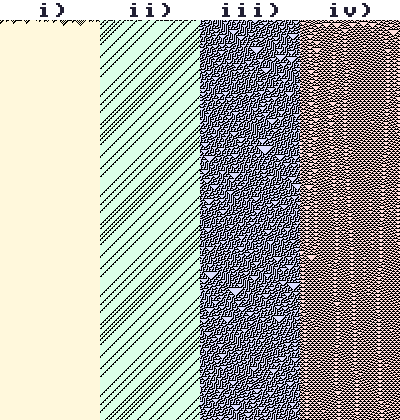
\includegraphics[width=\textwidth]{Images/P4/4classes.png}
    \caption{Representation of the four classes of elementary cellular automata according to Wolfram. Different colors represent the state $0$ at each class. ) Class-$1$ with Rule-$40$, the automaton quickly goes to a fixed state where all cells are $0$. ) Class-$2$ with Rule-$6$, the automaton quickly evolves to a periodic state. ) Class-$3$ with Rule-$30$, the automaton results in chaotic patterns that does not repeat. ) Class-$4$ with Rule-$54$, different regions can be appreciated before a periodic state is found (for longer times) . The initial cells (top) have a 50\% chance of being $0$ or $1$ and the automaton is iterated using a periodic boundary. }
    \label{fig:4classes}
\end{figure}





\begin{figure}
    \centering
    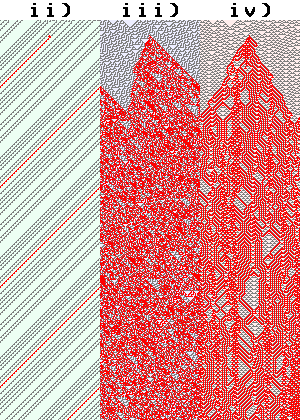
\includegraphics[width=\linewidth]{Images/P4/4classesDiffPatt.png}
    \caption{Difference Pattern in red for Class-$2$, Rule-$6$ (ii); in Class-$3$, Rule-$30$ (iii); and in Class-$4$, Rule-$54$ (iv).}
    \label{fig:4classDiffPatt}
\end{figure}







\clearpage



\begin{figure}
    \centering
    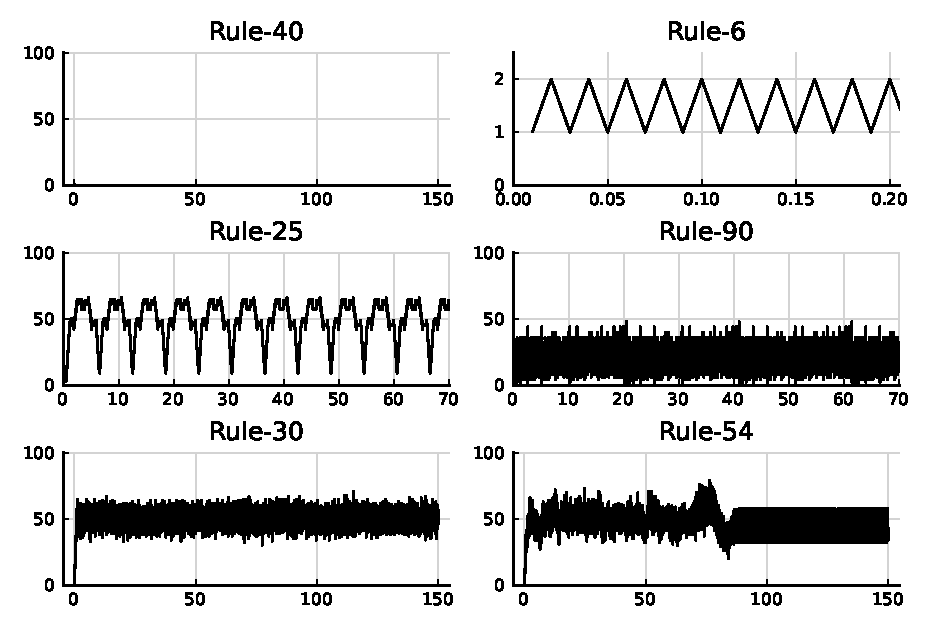
\includegraphics[width=\textwidth]{Images/P4/HammingTimeSeries.eps}
    \caption{For 6 different rules belonging to: Class-$1$ (Rule-$40$), Class-$2$ subclass LP (Rule-$6$), Class-$2$ subclass HP (Rule-$25$), Class-$3$ subclass U (Rule-$90$), Class-$3$ subclass C (Rule-$30$) and Class-$4$ subclass T (Rule-$54$); we represent the Hamming distance over time. The horizontal axis is in units of $L=100$ iterations, which is the size of the population.}
    \label{fig:HammDistTimeSeries}
\end{figure}


\begin{figure}
    \centering
    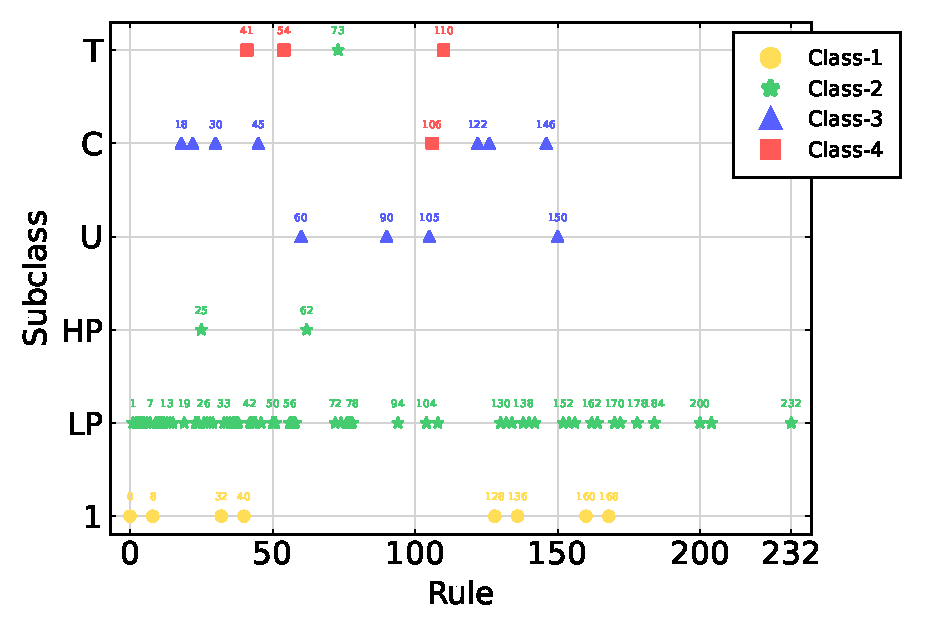
\includegraphics[width=\linewidth]{Images/P4/HammingClass.eps}
    \caption{Hamming distance classification. Colors and symbols correspond to Wolfram's classification, while position at the vertical axis correspond to the subclasses.}
    \label{fig:HammDistClass}
\end{figure}



\section{Hamming distance classification}

A way to observe how susceptible a given rule is to minimal changes in the initial conditions are the difference patterns. Each class has characteristic differences when comparing its difference patterns. As we can see in Fig.~\ref{fig:4classDiffPatt} the difference pattern for Class-$1$ is null, periodic for Class-$2$, noisy for Class-$3$ and complex for Class-$4$. In our study we have focused our attention in the number of cells that are different at each iteration. This is, again, the Hamming distance, which we used in the previous chapter. Here we obtain the Hamming distance of two initially close configurations varying only in one cell versus time, and analyze the saturated time series instead of the growth. 


We show the Hamming distance for $6$ rules that present different behavior in Fig.~\ref{fig:HammDistTimeSeries}. We have grouped together all rules that present the same behavior in a sub-classification of Wolfram's classification. The subclass column in Table~\ref{tab:ECAclasses} and Fig.~\ref{fig:HammDistClass} collects this information. Different initial conditions may produce a time series with different behavior. To help us to asses how complex can a rule get, we have classified the rule taking into account the time series with the most complex behaviour along $100$ different computations.

For Wolfram Class-$1$, the Hamming distance time series at this class goes rapidly to $0$. 

For Class-$2$ the time series varies periodically or is constant. We have subclass LP for low periods of no more than $20$ iterations, though most have period lesser than $5$; and HP for high periods greater or around $5L$ iterations. We can obtain the period o the series through its autocorrelation.

In Class-$3$ we have subclass U and C. Rules in subclass C give chaotic time series. Whereas those in subclass U have exactly the same time series for all initial conditions. The series is periodic, but with an extremely long period of exactly $2046$ iterations. This is very close to a power of $2$, $2^11 = 2048$. In fact with different values of $L$ one obtains that the periods of the Hamming distance are approximate to different powers of $2$. What is more, if the populations size is set to a power of $2$, the Hamming distance goes to $0$ after some iterations. Looking at Fig.~\ref{fig:Rule90}, where we represent the difference pattern for Rule-$90$, which it is the same than the pattern of evolution, we see that the patterns scale and repeat at periods that get multiplied by $2$. This is due to the auto-similarity that charactherizes this patterns as fractal.
As we explain below, all rules in subClass-$U$ are intrinsically fractal.




\begin{figure}
    \centering
    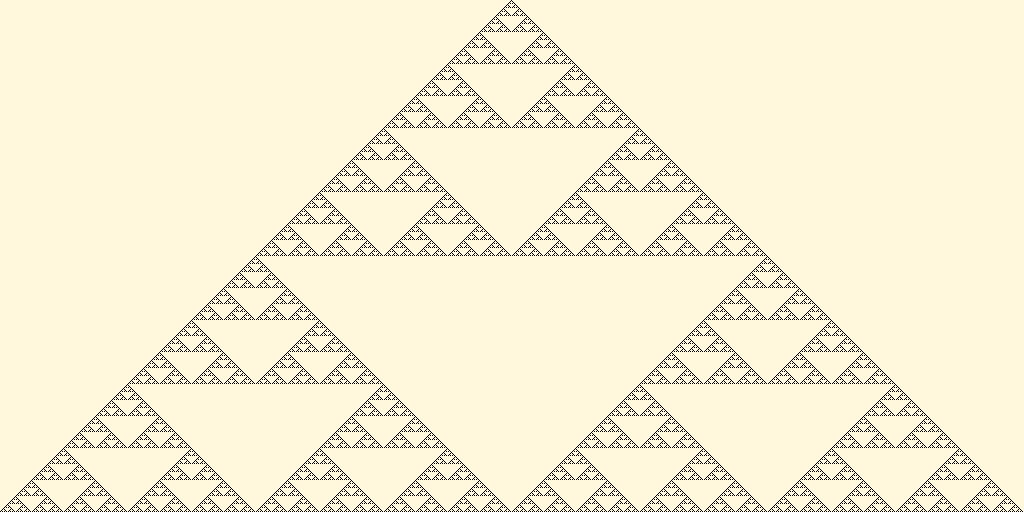
\includegraphics[width=\linewidth]{Images/P4/Sierpinski.png}
    \caption{Evolution of the ECA Rule-$90$ of size $1024$ starting with a single black cell, i.e. a $1$, at the center. If instead there is a single $0$ at the beginning, it gives the same result except with a black line at the top. This figure matches exactly with the difference pattern between two ECA's of the same rule and size where, after a brief transient (one iteration is enough), the state of the central cell is altered to be a $1$. The ECA forms a fractal named Sierpiński triangle.}
    \label{fig:Rule90}
\end{figure}




Class-$3$ automata evolve to complex patterns, so the fact that all initial conditions produce the same time series, is hard to believe. We can explain it analysing an intrinsic characteristic of these rules. For this explanation we will consider Rule-$90$ and its truth table from Table~\ref{tab:Rule90}. The rest of rules in this subclass have the same explanation. Choose any row from the table. If that row has a $0$ at the right side, then altering any of the trios at the left side of any row by adding modulo $2$ the trio of the row you chose would not alter the result on the right. If instead it had a $1$ at the right, the it would indeed alter the result. The rule itself is fractal. These only happens with rules in subclass U and marks the fractal behaviour of these rules, since, for these rules the evolution of a single $1$ in a sea of $0$s or vice-versa produces a fractal pattern like in Fig.~\ref{fig:Rule90}, that is exactly the same as the difference pattern of the rule with any initial condition.

Finally Class-$4$ is represented by subclass T, in which rules present transient chaos in the Hamming distance time series. The chaotic regime holds while there is complex behavior in the patterns and finishes when the evolution saturates in a periodic state.



\begin{figure}
    \centering
    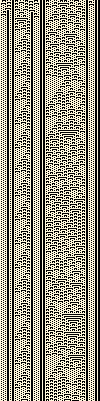
\includegraphics[height=0.95\textheight]{Images/P4/73.png}
    \caption{Time evolution of Rule-$73$ over $400$ iterations. Besides being classified as Class-$2$ in \textit{WolframAlpha}, this patterns belong to Class-$4$ more accurately.}
    \label{fig:Rule73}
\end{figure}





Each subclass belongs to one Wolfram class as appears on \textit{WolframAlpha} except for two rules. This is the case for Rule-$73$, which belongs to Wolfram Class-$2$ but subclass T. The rule was classified in this subclass because in one, and only one, of the $100$ time series we saw transient chaos. In Fig.~\ref{fig:Rule73} we see an evolution pattern that could be classified to Wolfram Class-$4$, but this behaviour happens in rare occasions. Rules in the $HP$ subclass are close to being from subClass-$T$ also, but since the times where the patterns are complex are very narrow, we did not detect transient chaos.

Rule-$106$ is also an exception. We have classified it as subclass C whereas in \textit{WolframAlpha} is classified as Class-$4$. Watching the pattern evolution in Fig.~\ref{fig:Rule106} we clearly see this is an error, as the patterns looks more akin to those in Class-$3$.




\begin{figure}
    \centering
    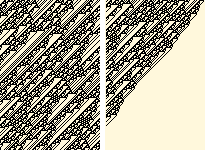
\includegraphics[width=\linewidth]{Images/P4/106.png}
    \caption{Time evolution of Rule-$106$. At the left, the evolution under periodic boundary conditions shows patterns that never repeat for long times like those at Class-$3$. At the right, evolved under a fixed boundary, the zeros propagate to the left until all cells are zero, making it fall under definition of Class-$1$.}
    \label{fig:Rule106}
\end{figure}



\section{Discussion and conclusions}

We have made an algorithm that classifies the ECA rules analyzing a time series instead of analyzing an image. Thus requires less quantity of data to analyze than Wolfram method, so it is more effective. The classification separates the rules in the same classes save for some arguably misclassified rules in the \textit{WolframAlpha} engine. This is not a setback  because Wolfram's classification was subject of variance given different initial conditions.

With the autocorrelation of the Hamming distance we can also obtain its period, but this is not generally the period of the cellular automaton, and has a strong dependence with populations size.


\begin{thebibliography}{04}


\bibitem{VonNeummanCA}
\raggedright
J. von Neumann, A. W. Burks, 
Theory of Self-Reproducing Automata. 
University of Illinois Press (1966).
\url{https://cdn.patentlyo.com/media/docs/2012/04/VonNeumann.pdf}



\bibitem{PhysicsCA1}
\raggedright
D. Chowdhury, L. Santen, and A. Schadschneider,
Statistical physics of vehicular traffic and some related systems.
Phys. Rep. \textbf{329}, 199--329 (2000).
\url{https://doi.org/10.1016/S0370-1573(99)00117-9}


\bibitem{PhysicsCA2}
\raggedright
C. Burstedde, K. Klauck, A.Schadschneider, and J. Zittartz,
Simulation of pedestrian dynamics using a two-dimensional cellular automaton. 
Physica A \textbf{295}, 507--525 (2001).
\url{https://doi.org/10.1016/S0378-4371(01)00141-8}

\bibitem{PhysicsCA3}
\raggedright
D. H. Rothman and J. M. Keller,
Immiscible cellular-automaton fluids.
J. Stat. Phys. \textbf{52}, 1119--1127 (1988). 
\url{https://doi.org/10.1007/BF01019743}

\bibitem{PhysicsCA4}
\raggedright
L. Kadanoff, S. R. Nagel, L. Wu, and S. Zhou,
Scaling and universality in avalanches.
Phys. Rev. A \textbf{39}, 6524 (1989).
\url{https://doi.org/10.1103/PhysRevA.39.6524}

\bibitem{PhysicsCA5}
\raggedright
D. A. Meyer,
From quantum cellular automata to quantum lattice gases.
J. Stat. Phys. \textbf{85}, 551--574 (1996).
\url{}

\bibitem{EngineeringCA1}
\raggedright
P. Tougaw, L. Douglas, and S. Craig,
Logical devices implemented using quantum cellular automata.
J. Appl. Phys. \textbf{75}, 1818--1825 (1994).
\url{https://doi.org/10.1007/BF02199356}

\bibitem{CryptographyCA1}
\raggedright
S. Nandi, B. K. Kar, and P. Pal Chaudhuri,
Theory and applications of cellular automata in cryptography.
IEEE Trans Comput \textbf{43} 1346--1357 (1994).
\url{https://doi.org/10.1109/12.338094}

\bibitem{CryptographyCA2Lya}
\raggedright
J. Machiacao, A. G. Marco, and O. M. Bruno,
Chaotic encryption method based on life-like cellular automata.
\textbf{39}, 12626--12635 (2012).
\url{https://doi.org/10.1016/j.eswa.2012.05.020}

\bibitem{BiologyCA1}
\raggedright
J. Lechleiter, S. Girard, E. Peralta, and D. Clapham,
Spiral calcium wave propagation and annihilation in Xenopus laevis oocytes.
Science \textbf{252}, 123--126 (1991).
\url{https://doi.org/10.1126/science.2011747}

\bibitem{BiologyCA2}
\raggedright
K. C. De Carvalho and T. Tomé,
Probabilistic cellular automata describing a biological two-species system.
Mod. Phys. Lett. B \textbf{18}, 873--880 (2004).
\url{https://doi.org/10.1142/S0217984904007396}

\bibitem{BiologyCA3}
\raggedright
M. Redeker, A. Adamatzky, and G. J. Martínez,
Expressiveness of elementary cellular automata.
Int J Mod Phys C \textbf{24}, 1350010 (2013).
\url{https://doi.org/10.1142/S0129183113500101}



\bibitem{WolframCA_ClassOrigen}
\raggedright
S. Wolfram,
Universality and complexity in cellular automata.
Physica D \textbf{10}, 1--35 (1984).
\url{https://doi.org/10.1016/0167-2789(84)90245-8}

\bibitem{UniversalComputingECA110}
\raggedright
M. Cook,
Universality in Elementary Cellular Automata.
Complex Syst. \textbf{15}, 1--40 (2004). 
\url{https://content.wolfram.com/sites/13/2018/02/15-1-1.pdf}
\end{thebibliography}


